% Preamble templated from Dhawal24112006/EE1030
\documentclass{beamer}
\mode<presentation>
\usepackage{amsmath}
\usepackage{amssymb}
\usepackage{adjustbox}
\usepackage{subcaption}
\usepackage{multicol}
\usepackage{mathtools}
\usepackage{listings}
\usepackage{url}

\usetheme{Boadilla}
\usecolortheme{lily}
\setbeamertemplate{footline}
{
  \leavevmode%
  \hbox{%
  \begin{beamercolorbox}[wd=\paperwidth,ht=2.25ex,dp=1ex,right]{author in head/foot}%
    \insertframenumber{} / \inserttotalframenumber\hspace*{2ex}
  \end{beamercolorbox}}%
  \vskip0pt%
}
\setbeamertemplate{navigation symbols}{}

% Custom Commands
\providecommand{\abs}[1]{\left\vert#1\right\vert}
\providecommand{\norm}[1]{\lVert#1\rVert}

\lstset{
frame=single,
breaklines=true,
columns=fullflexible,
showstringspaces=false
}

\numberwithin{equation}{section}

\title{POMPS Presentation: 1.2.55}
\author{Subhodeep Chakraborty \\ ee25btech11055,\\IIT Hyderabad.}
\date{\today}

\begin{document}

\begin{frame}
\titlepage
\end{frame}

\section*{Outline}
\begin{frame}
\tableofcontents
\end{frame}

\section{Problem}
\begin{frame}
\frametitle{Problem Statement}
\textbf{Question:} 
\vspace{0.5cm}

The minimum number of terms required in $e^x$ series expansion to evaluate at $x = 1$ correct up to 3 decimal places is:
\begin{multicols}{4}
  \begin{enumerate}
    \item 8
    \item 7
    \item 6
    \item 5
  \end{enumerate}
\end{multicols}
\end{frame}

\section{Solution}
\begin{frame}{Matrix Operator Representation}
Let $\mathbf{S}$ be the infinite-dimensional downshift matrix, representing a discrete unit delay operator ($z^{-1}$). 
\vspace{0.5cm}

When multiplied by a vector, it shifts all elements down by one position:
\begin{equation}
    \mathbf{S} = \begin{bmatrix} 0 & 0 & 0 & \dots \\ 1 & 0 & 0 & \dots \\ 0 & 1 & 0 & \dots \\ \vdots & \vdots & \ddots & \ddots \end{bmatrix}, \quad \mathbf{S} \begin{bmatrix} a \\ b \\ c \\ \vdots \end{bmatrix} = \begin{bmatrix} 0 \\ a \\ b \\ \vdots \end{bmatrix}
\end{equation}
\end{frame}

\begin{frame}{Ideal System Response}
The ideal infinite impulse response of this system is generated by applying the matrix exponential to an impulse vector $\mathbf{\delta} = [1, 0, 0, \dots]^T$.
\vspace{0.5cm}

Expanding the Taylor series of $e^{\mathbf{S}}$ directly generates the Maclaurin coefficients:
\begin{equation}
    \mathbf{h}_{\text{ideal}} = e^{\mathbf{S}} \mathbf{\delta} = \left( \mathbf{I} + \mathbf{S} + \frac{1}{2!} \mathbf{S}^2 + \frac{1}{3!} \mathbf{S}^3 + \dots \right) \begin{bmatrix} 1 \\ 0 \\ 0 \\ \vdots \end{bmatrix} = \begin{bmatrix} 1 \\ 1 \\ 1/2! \\ 1/3! \\ \vdots \end{bmatrix}
\end{equation}
\end{frame}

\begin{frame}{Filter Truncation and Error Matrix}
Truncating this infinite system to a finite filter length $N$ yields the error matrix, $\mathbf{E}_N$:
\begin{equation}
    \mathbf{E}_N = \sum_{k=N}^{\infty} \frac{1}{k!} \mathbf{S}^k
\end{equation}
\vspace{0.3cm}

To measure the maximum size of this error, we apply the induced $l_1$-norm ($\norm{\cdot}_1$), defined as the maximum absolute column sum of a matrix. We use this instead of Frobenius as we have an infinite matrix and this norm looks for worst-case scenario in each column.
\end{frame}

\begin{frame}{Applying the Induced $l_1$-Norm}
Because every column of $\mathbf{S}$ contains exactly one $1$ and zeros elsewhere, its column sum is strictly $1$, hence $\norm{\mathbf{S}}_1 = 1$.
\vspace{0.3cm}

By the multiplicative property of norms ($\norm{\mathbf{A}\mathbf{B}} \le \norm{\mathbf{A}}\norm{\mathbf{B}}$), we establish:
\begin{equation}
    \norm{\mathbf{S}^k}_1 \le \norm{\mathbf{S}}_1^k = 1^k = 1
\end{equation}

This allows us to bound the error:
\begin{equation}
    \norm{\mathbf{E}_N}_1 \le \sum_{k=N}^{\infty} \frac{\norm{\mathbf{S}}_1^k}{k!} = \sum_{k=N}^{\infty} \frac{1}{k!}
\end{equation}
\end{frame}

\begin{frame}{Bounding the Error}
Expanding the summation and factoring out the first neglected term, $\frac{1}{N!}$, yields:
\begin{align}
    \norm{\mathbf{E}_N}_1 &\le \frac{1}{N!} + \frac{1}{(N+1)!} + \frac{1}{(N+2)!} + \dots \\
    \norm{\mathbf{E}_N}_1 &\le \frac{1}{N!} \left( 1 + \frac{1}{N+1} + \frac{1}{(N+1)(N+2)} + \dots \right)
\end{align}
\end{frame}

\begin{frame}{Constructing an Algebraic Bound}
To construct a solvable algebraic bound, we replace the increasing denominators with the worst-case constant, $N$, as $\frac{1}{N+1} < \frac{1}{N}$.
\vspace{0.3cm}

This substitution results in a standard infinite geometric series:
\begin{equation}
    \norm{\mathbf{E}_N}_1 \le \frac{1}{N!} \left( 1 + \frac{1}{N} + \frac{1}{N^2} + \dots \right) = \frac{1}{N!} \sum_{m=0}^{\infty} \left(\frac{1}{N}\right)^m
\end{equation}
\begin{equation}
    \norm{\mathbf{E}_N}_1 \le \frac{1}{N!} \left( \frac{1}{1 - 1/N} \right) = \frac{1}{N!} \left( \frac{N}{N-1} \right)
\end{equation}
\end{frame}
\begin{frame}{Defining Error Tolerance}
The problem requires the evaluation to be correct up to 3 decimal places.
\vspace{0.3cm}

To guarantee this precision, the absolute truncation error must be strictly less than half of the place value of the third decimal digit ($10^{-3}$).
\vspace{0.5cm}

Therefore, our target error tolerance ($\epsilon$) is bounded by:
\begin{equation}
    \epsilon \le \frac{1}{2} \times 10^{-3} = 0.0005
\end{equation}
\vspace{0.5cm}

\end{frame}
\begin{frame}{Enforcing Tolerance Limits}
For 3 decimal places of precision, we apply error tolerance ($\epsilon \le 0.0005$) on our derived bound:
\begin{equation}
    \frac{1}{N!} \left( \frac{N}{N-1} \right) \le 0.0005
\end{equation}

Checking values of the filter length $N$:
\begin{align}
    N &= 5: \quad \frac{1}{120} \left( \frac{5}{4} \right) = \frac{1}{96} \approx 0.01042 \quad (\text{Not met}) \\[10pt]
    N &= 6: \quad \frac{1}{720} \left( \frac{6}{5} \right) = \frac{1}{600} \approx 0.00166 \quad (\text{Not met}) \\[10pt]
    N &= 7: \quad \frac{1}{5040} \left( \frac{7}{6} \right) = \frac{7}{30240} \approx 0.00023 \quad (\text{Met})
\end{align}
\end{frame}
\begin{frame}{Comparison with Classical Lagrange Bound}
The standard method to solve this question is to use Lagrange Error Bound for $N$ terms (highest power $n = N-1$):
\begin{equation}
    R_{N-1}(x) = \frac{e^c}{N!} x^N \quad \text{where } c \in (0,1)
\end{equation}
Evaluating at $x=1$ and knowing $e < 3$, the classical upper bound is:
\begin{equation}
    R_{N-1}(1) < \frac{3}{N!}
\end{equation}

Testing our derived answer of $N=7$:
\begin{equation}
    R_6(1) < \frac{3}{5040} \approx 0.000595
\end{equation}
\textbf{Result:} The classical bound fails at our $\le 0.0005$ tolerance. Our derived bound ($\approx 0.00023$) is significantly tighter, proving $N=7$ is sufficient. Thus, due to having to guess an upper limit for $e$, the classical method performs worse than our method. (In fact, taking exact value of $e$ also yields $0.000539$, which is still above the threshold)
\end{frame}
\begin{frame}{Conclusion}
Thus minimum number of required terms is 7.
\vspace{0.3cm}

The Maclaurin series for $e^x$ evaluated at $x = 1$ is:
\begin{equation}
    e^1 = \sum_{k=0}^{\infty} \frac{1}{k!} = 1 + 1 + \frac{1}{2!} + \frac{1}{3!} + \dots
\end{equation}

If we take $N$ terms, the sum stops at the index $k = N-1$:
\begin{equation}
    S_N = \sum_{k=0}^{N-1} \frac{1}{k!}
\end{equation}

Our target of $N=7$ terms expands to a 6th-degree polynomial:
\begin{equation}
    S_7 = \underbrace{1}_{k=0} + \underbrace{1}_{k=1} + \underbrace{\frac{1}{2!}}_{k=2} + \underbrace{\frac{1}{3!}}_{k=3} + \underbrace{\frac{1}{4!}}_{k=4} + \underbrace{\frac{1}{5!}}_{k=5} + \underbrace{\frac{1}{6!}}_{k=6} = 2.7181
\end{equation}
\end{frame}
\section{Python Codes}
\begin{frame}[fragile,allowframebreaks]{Python Implementation}
\begin{lstlisting}[basicstyle=\scriptsize\ttfamily][language=Python]
import numpy as np
import matplotlib.pyplot as plt
from scipy.special import factorial

e_val = np.exp(1)

# start at 3 to avoid div by zero in the N/(N-1) bound
N = np.arange(3, 11)

errs = []
bounds = []

for n in N:
    k = np.arange(n)
    approx = np.sum(1 / factorial(k))
    
    errs.append(np.abs(e_val - approx))
    bounds.append((1 / factorial(n)) * (n / (n - 1)))

plt.figure(figsize=(9, 5))

plt.plot(N, errs, marker='o', label='Actual Error')
plt.plot(N, bounds, marker='s', ls='--', label='Theoretical Bound')

plt.axhline(y=0.0005, color='r', ls=':', label='Tolerance (0.0005)')
plt.axvline(x=7, color='g', ls=':', alpha=0.5)

plt.annotate('N=7', xy=(7, 0.0005), xytext=(7.3, 0.005),
             arrowprops=dict(facecolor='black', shrink=0.05, width=1, headwidth=5))

plt.yscale('log')
plt.xlabel('Number of terms (N)')
plt.ylabel('Error')
plt.title('Truncation Error for e^x at x=1')
plt.xticks(N)
plt.grid(True, ls="--", alpha=0.4)
plt.legend()

plt.tight_layout()
path='../figs/plot.png'
plt.savefig(path, dpi=300)
print(f"Saved: {path}")
plt.close()
\end{lstlisting}
\end{frame}

\section{Plot}
\begin{frame}{Error Plot}
    \begin{figure}[h]
        \centering
        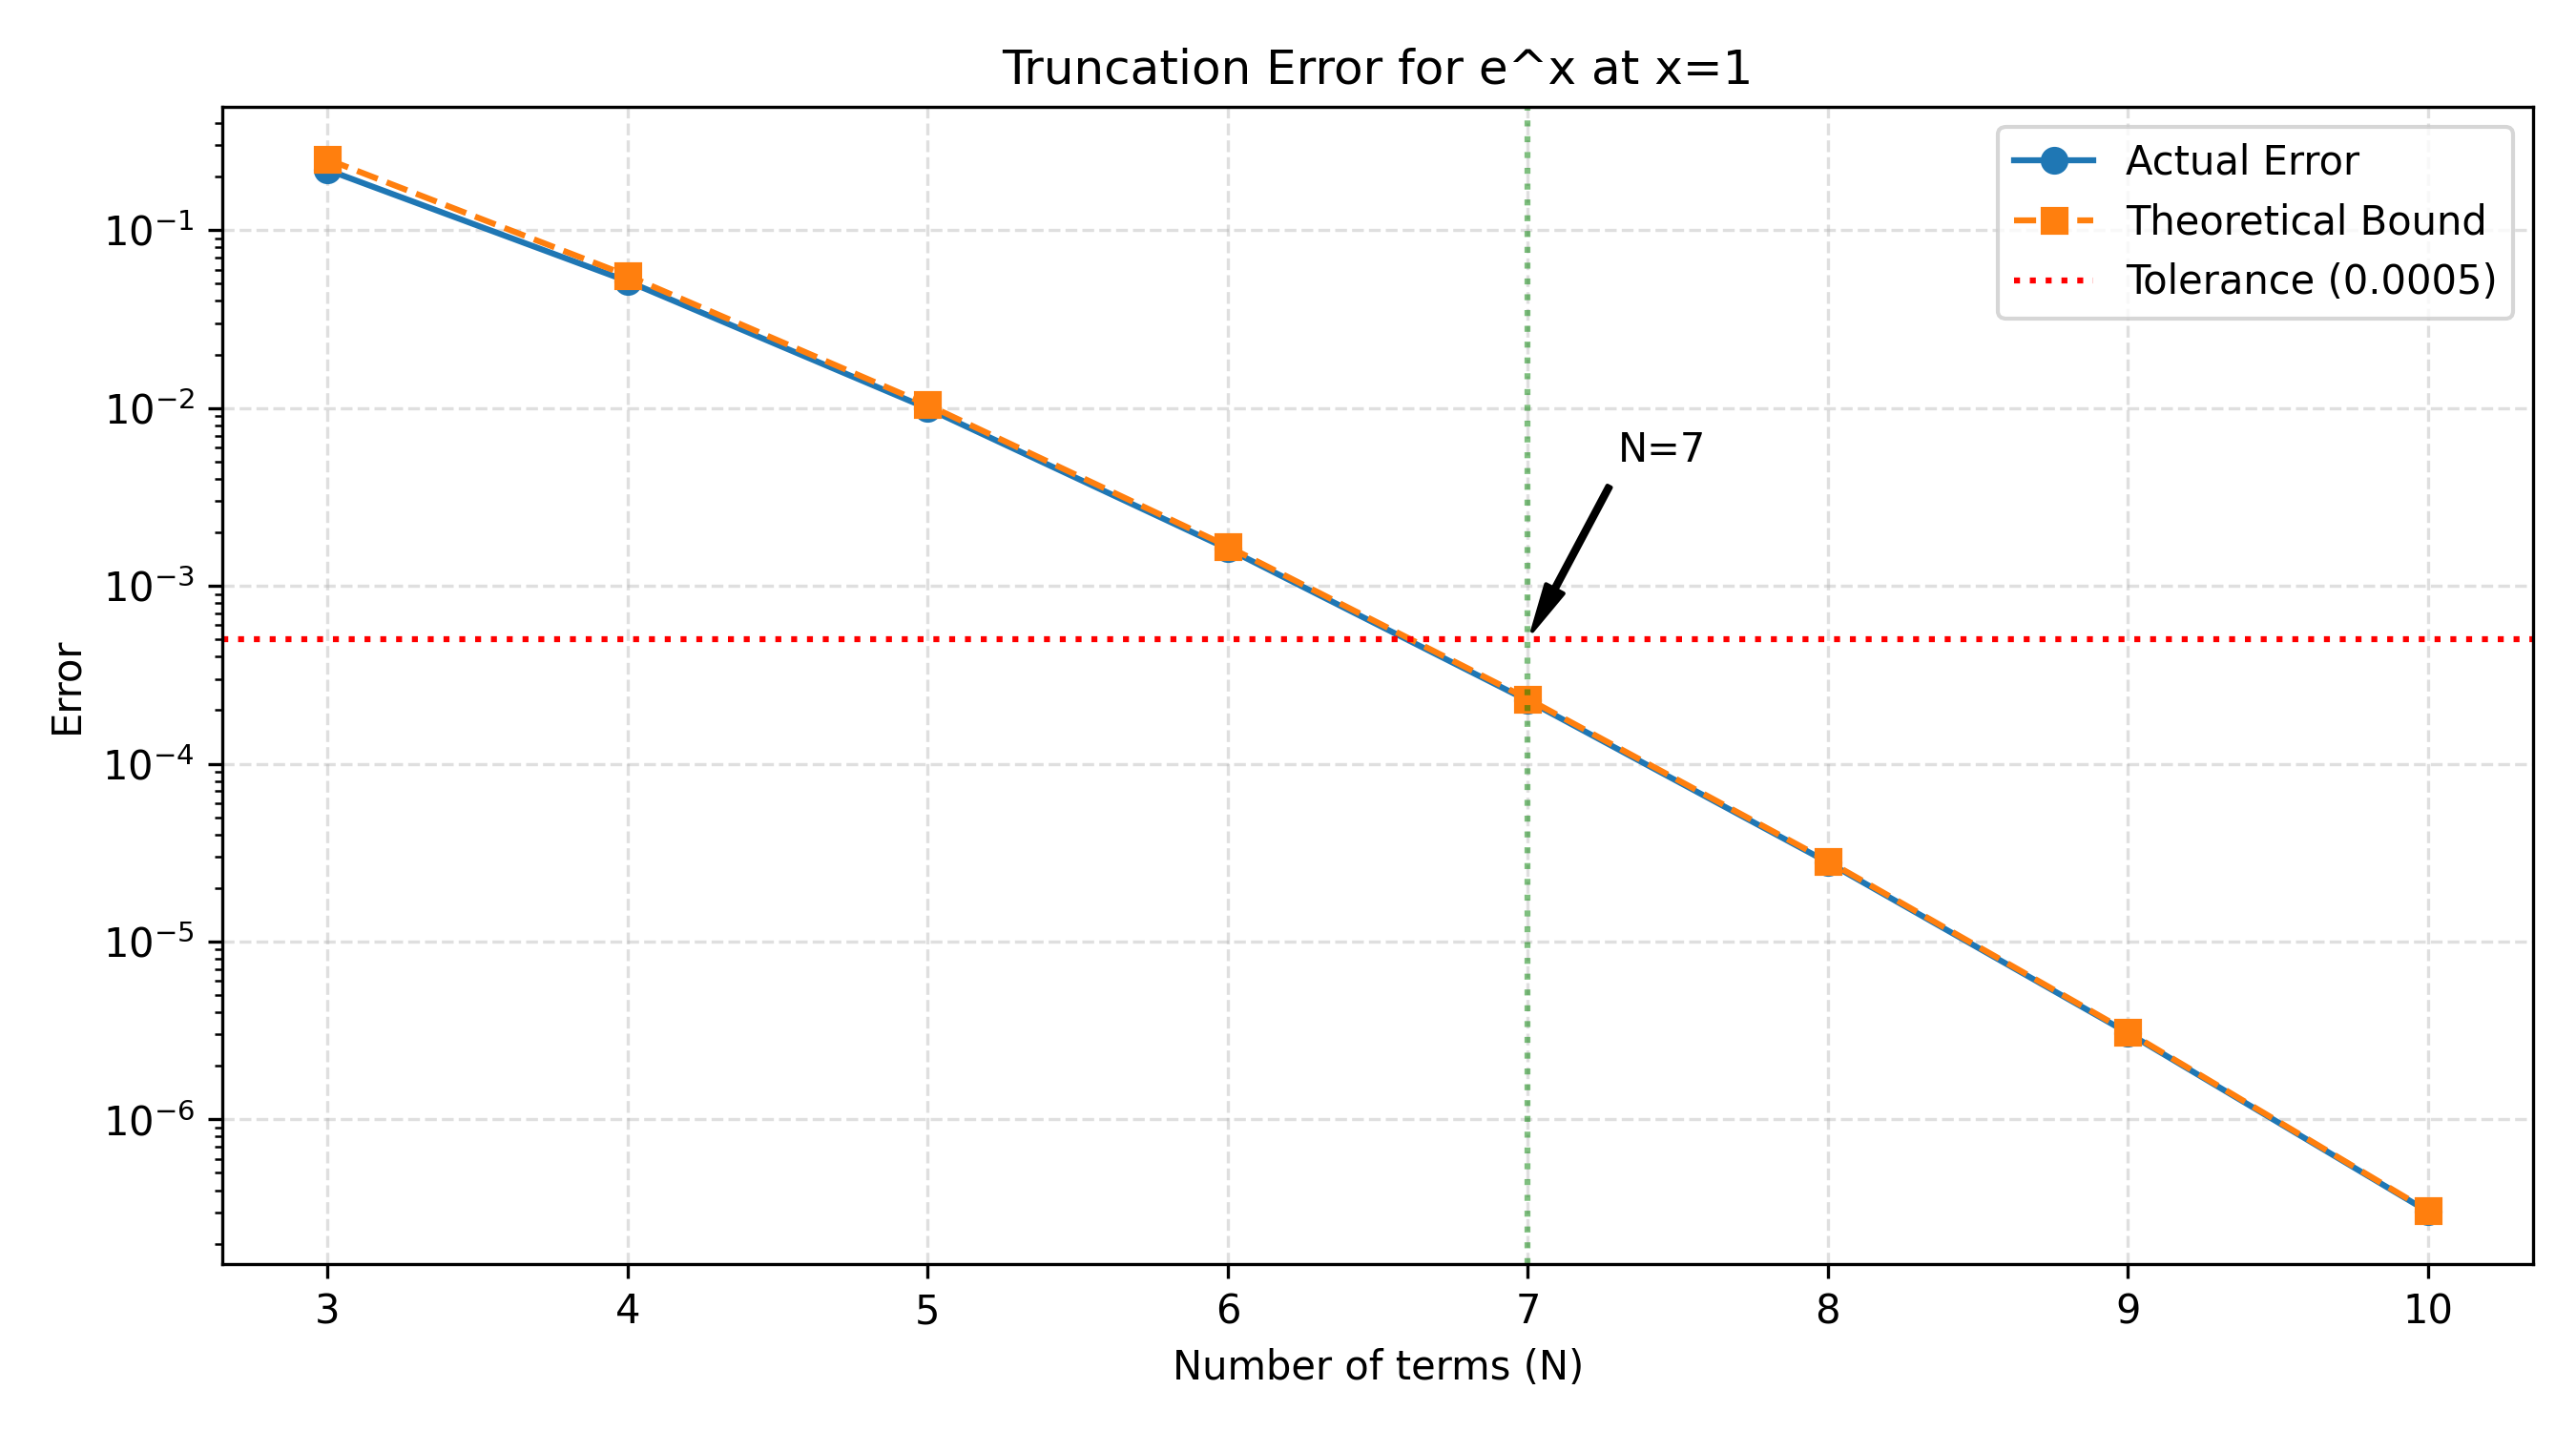
\includegraphics[width=0.85\linewidth]{../figs/plot.png}
        \caption{Error v/s N}
    \end{figure}
\end{frame}
\end{document}
